\documentclass[aspectratio=169]{beamer}
\usepackage[utf8]{inputenc}
\usepackage{multicol}
\usepackage[czech]{babel}
\usepackage{amsmath}
\usepackage{csquotes}

\usepackage[sfdefault]{roboto}
\usepackage[T1]{fontenc}

\title{Prohlížeče, nebezpečí internetu a autorský zákon}
\date{WBA | 3., 4. hodina}
\author[Cajthaml]{Matěj Cajthaml}

\usetheme{material}

\usePrimaryCustom

\begin{document}

\begin{frame}
\titlepage
\end{frame}

\begin{frame}{Obsah prezentace}
    \begin{cardTiny}
        \begin{minipage}{\textwidth}
            \vspace{1ex}
            \tableofcontents
        \end{minipage}
    \end{cardTiny}
\end{frame}



\section{Opakování}

\begin{frame}{Opakování 1}
    \begin{cardTiny}
        \begin{center}
            \textbf{Kolik uzlů měla síť ARPANET při založení?}
        \end{center}
    \end{cardTiny}
    \begin{cardTiny}
        \begin{center}
            \textbf{Kolik zařízení bylo připojeno k internetu v roce 2009?}
        \end{center}
    \end{cardTiny}
       
    \begin{cardTiny}
        \begin{center}
            \textbf{Jaké služby využívájí internet?}
        \end{center}
    \end{cardTiny} 
    \begin{cardTiny}
        \begin{center}
            \textbf{Jaký je rozdíl mezi HTTP a HTTPS?}
        \end{center}
    \end{cardTiny}
\end{frame}

\begin{frame}{Opakování 2}
    \begin{cardTiny}
        \begin{center}
            \textbf{K čemu slouží DNS?}
        \end{center}
    \end{cardTiny}
    \begin{cardTiny}
        \begin{center}
            \textbf{Jaký je rozdíl mezi webovým vyhledávačem a katalogem?}
        \end{center}
    \end{cardTiny}
    \begin{cardTiny}
        \begin{center}
            \textbf{Co je to temný internet?}
        \end{center}
    \end{cardTiny}
    \begin{cardTiny}
        \begin{center}
            \textbf{Co je to tzv. hypertextový dokument?}
        \end{center}
    \end{cardTiny}
\end{frame}

\begin{frame}{Určete části URL} 
    \begin{cardTiny}
        \begin{center}
            $ \overbrace{\text{https://}}^{\text{ }}
            \overbrace{\text{en.wikipedia.org/}}^{\text{ }}
            \overbrace{\text{wiki/IPv6/}}^{\text{ }}
            \overbrace{\text{\#Security}}^{\text{ }} $
        \end{center}
    \end{cardTiny}
\end{frame}



\section{Nebezpečí na internetu}

\begin{frameImg}[width]{img/webdanger.png}
    \vspace*{60mm}
    \begin{cardTiny}
        \vspace*{\fill}
        \begin{center}
            \textbf{Nebezpečí na internetu}
        \end{center}
    \end{cardTiny}
\end{frameImg}

\begin{frame}{Co se Vám může stát?}
    \begin{cardTiny}
        \begin{center}
            \textbf{Co se Vám může na internetu stát?}
        \end{center}
    \end{cardTiny}
\end{frame}

\begin{frame}{Nebezpečí na internetu}
    \begin{cardTiny}
        \begin{flushleft}
            Závislost na internetu.

            Zneužití osobních informací (údaje, fotografie, pozice, ...).

            Zneužití záznamů webkamery a zvuku.

            Podvody - ztráta majetku, peněz.

            Ztráta dat / zablokování zařízení.
        
            Kyberšikana.
        \end{flushleft}
    \end{cardTiny}
    \begin{cardTiny}
        \begin{flushleft}
            \textbf{Na internetu se nachází spousta divných (i nelegálních) věcí. I to je nebezpečí. \href{https://www.youtube.com/watch?v=dQw4w9WgXcQ}{ODKAZ}}
        \end{flushleft}
    \end{cardTiny}
\end{frame}

\begin{frame}{Malware}
    \begin{cardTiny}
        \begin{flushleft}
            = \textbf{Mal}icious Soft\textbf{ware}

            \vspace{2ex}
            Nevyžádaný software - program.

            Určen k poškození počítače či uživatele.

            \vspace{2ex}        
            Např. viry, trojské koně, spyware, adware, ...
        \end{flushleft}
    \end{cardTiny}
\end{frame}

\begin{frame}
    \begin{multicols}{2}
        \centering

        \begin{cardTiny}
            \begin{flushleft}
                \textbf{Virus}

                Samovolně se šíří bez vědomí uživatele. Obtěžuje, níčí data, šíří se. Např. e-maily, přenosná media.
            \end{flushleft}
        \end{cardTiny}

        \begin{cardTiny}
            \begin{flushleft}
                \textbf{Trojský kůň}

                Škodlivá část je skryta v nezávadném programu. Uživatel nezjistí zda se jedná o trojského koně. Sleduje aktivitu, zadávání klávesnice a informace odesílá.
            \end{flushleft}
        \end{cardTiny}

        \begin{cardTiny}
            \begin{flushleft}
                \textbf{Adware}

                Zobrazuje nevyžádané reklamy, pop-up okna, falešené ikony.
            \end{flushleft}
        \end{cardTiny}

        \begin{cardTiny}
            \begin{flushleft}
                \textbf{Spyware}

                Určen k sledování. Sleduje aktivitu a odesílá data.
            \end{flushleft}
        \end{cardTiny}

        \begin{cardTiny}
            \begin{flushleft}
                \textbf{Počítačový červ}

                Šíří se po síti bez vědomí uživatele. Může např. mazat soubory a to např. až při aktivací útočníkem.
            \end{flushleft}
        \end{cardTiny}

        \begin{cardTiny}
            \begin{flushleft}
                \textbf{Ransomware}

                Zašifruje data počítače a nutí uživatele zaplatit nesmyslnou částku (v kryptoměně) pro odblokování dat.
            \end{flushleft}
        \end{cardTiny}
    \end{multicols}
\end{frame}

\begin{frame}
    \begin{center}
        
\includegraphics[width=0.8\textwidth]{img/ransomware.jpg}
    \end{center}
\end{frame}

\begin{frame}{Malware}
    \begin{cardTiny}
        \begin{center}
            \textbf{Jaký malware je nejvíce nebezpečný?}
        \end{center}
    \end{cardTiny}
\end{frame}

\begin{frame}{Phishing}
    \begin{cardTiny}
        \begin{flushleft}
            \textbf{p}assword \textbf{h}arvesting f\textbf{ishing} = rhybaření

            \vspace{2ex}

            Podvodná technika používaná na internetu k získání citlivých údajů.

            Podvodné e-maily, bannery, \textbf{stránky}, SMS, hovory, administrátoři žádající zadávání údajů.

            \vspace{2ex}
            Velmi častý útok na internetu. Člověk se s ním setká všude v podstatě každý den.

            \vspace{2ex}
            \href{https://www.hoax.cz/phishing/}{https://www.hoax.cz/phishing/}
        \end{flushleft}
    \end{cardTiny}
    \begin{cardTiny}
        \begin{center}
            \textbf{Kdo je cílem těchto útoků?}
        \end{center}
    \end{cardTiny}
\end{frame}

\begin{frame}
    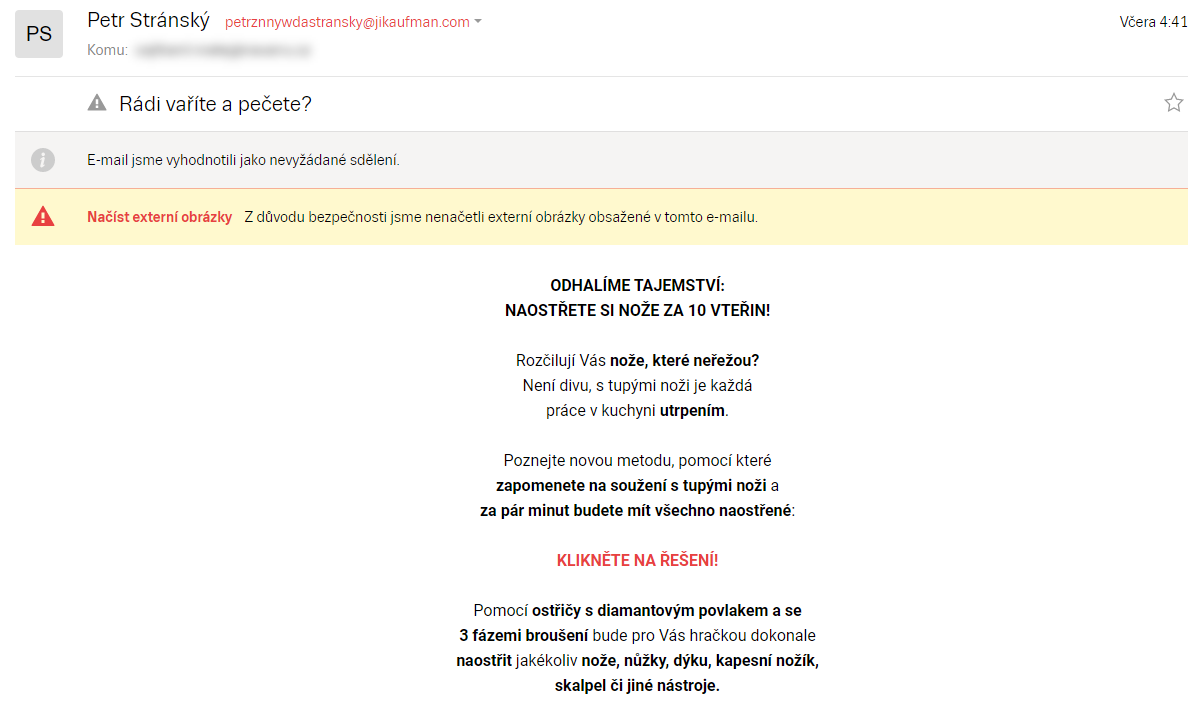
\includegraphics[width=\textwidth]{img/spam-1.png}
\end{frame}

\begin{frame}
    \begin{center}
        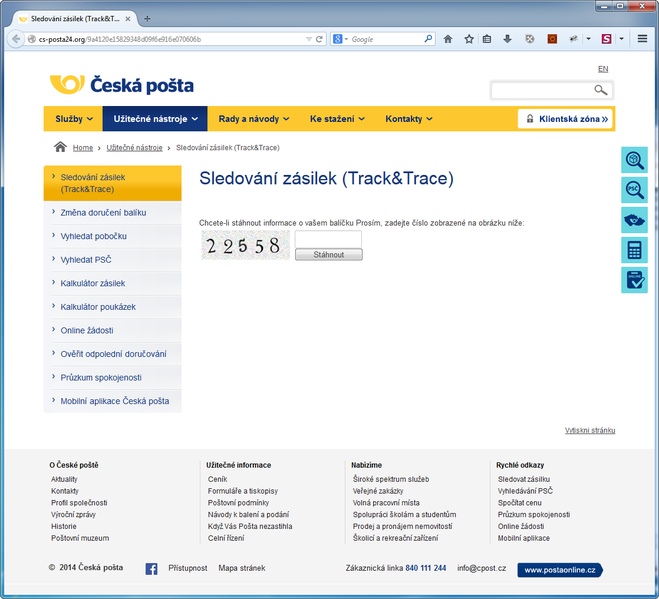
\includegraphics[width=0.7\textwidth]{img/posta.png}
    \end{center}
\end{frame}



\section{Ochrana proti nebezpečí}

\begin{frame}{Phishing}
    \begin{cardTiny}
        \begin{center}
            \textbf{Jak dále lze poznat phishing?}
        \end{center}
    \end{cardTiny}
    \begin{cardTiny}
        \begin{center}
            \textbf{Jak se bránit proti phishingu?}
        \end{center}
    \end{cardTiny}
\end{frame}

\begin{frame}{Ochrana proti nebezpečí na internetu}
    \begin{cardTiny}
        \begin{flushleft}
            Většina nebezpečí vzniká pokud to uživatel dovolí.

            Antivirové programy.

            Antimalwarové programy.

            Adware v freewarovém software.

            Podmínky při instalaci programů.

            Pravidelné aktualizace.

            Nestahovat a neklikat na neznáme soubory a odkazy (a emaily).

            Zkontrolovat certifikáty (důvěrné údaje pouze na HTTP\textbf{S}).
            
            Nepřihlašovat se z jiných než oficiálních stránek.
            
            Nezadávat důvěrná data na vyzvání.
        \end{flushleft}
    \end{cardTiny}
    \begin{cardTiny}
        \begin{center}
            \textbf{Jak se dá dále bránit?}
        \end{center}
    \end{cardTiny}
\end{frame}


\section{Digitální stopa}

\begin{frameImg}[width]{img/fingerprint.jpg}
    \vspace*{60mm}
    \begin{cardTiny}
        \vspace*{\fill}
        \begin{center}
            \textbf{Digitální stopa}
        \end{center}
    \end{cardTiny}
\end{frameImg}


\begin{frame}{Digitální stopa}
    \begin{cardTiny}
        \begin{flushleft}
            Digitální stopa = záznamy, co necháváme za sebou, když projíždíme internet.

            Jak na osobním zařízení tak i na serveru.

            Např. příspěvky, komentáře, nákupy, ...

            Cenné informace.

            \vspace{2ex}

            Vlastní - vědomá, nevědomá.

            Zanechaná (ne)příteli.
        \end{flushleft}
    \end{cardTiny}
    \begin{cardTiny}
        \begin{center}
            \textbf{Proč je digitální stopa tak cenná? Jak se dá zneužít?}
        \end{center}
    \end{cardTiny}
    \begin{cardTiny}
        \begin{center}
            \textbf{Jak se bránit/minimalizovat zanechávání stopy?}
        \end{center}
    \end{cardTiny}
\end{frame}

\begin{frame}{Metadata}
    \begin{cardTiny}
        \begin{flushleft}
            Metadata = data o datech.

            Informace o nějaké věci (soubor, fotka, příspěvek, email).

            Např. lokace, vytvoření, zařízení, komu se e-mail odeslal, odkuď, ...
        \end{flushleft}
    \end{cardTiny}
\end{frame}


\section{Webový prohlížeč}

\begin{frameImg}[width]{img/browsers.png}
    \vspace*{60mm}
    \begin{cardTiny}
        \vspace*{\fill}
        \begin{center}
            \textbf{Webový prohlížeč}
        \end{center}
    \end{cardTiny}
\end{frameImg}

\begin{frame}{Webový prohlížeč}
    \begin{cardTiny}
        \begin{flushleft}
            Software určený k prohlížení WWW - webů.

            Komunikace se servery pomocí protokolu HTTP a HTTPS.

            Obsahuje tzv. \textbf{vykreslovací (renderovavací) jádro}, které převádí kód do grafické podoby.

            \vspace{2ex}

            Nejznámější jádra:\\Trident (Internet Explorer)\\Gecko (Mozilla Firefox)\\WebKit (Google Chrome (Blink), Safari)
        \end{flushleft}
    \end{cardTiny}
    \begin{cardTiny}
        \begin{center}
            \textbf{Čím se tyto jádra liší?}
        \end{center}
    \end{cardTiny}
\end{frame}

\begin{frame}{Internet Explorer - Historie a přítomnost}
    \begin{cardTiny}
        \begin{flushleft}
            Již brzy přestane být podporovaný samotným Microsoftem.

            Plně ho nahradil Microsoft Edge, který stojí na \textbf{Chromium}.
        \end{flushleft}
    \end{cardTiny}
    \begin{cardTiny}
        \begin{flushleft}
            \textbf{Chromium}

            Jádro, které má Google Chrome.

            Staví z něho spousta nových prohlížečů (Vivaldi, Opera, MS Edge, Brave, ...).

            Lze využívat samotné Chromium - lehčí verze Google Chrome bez přihlašování, sledování a dalších věcí.     
        \end{flushleft}
    \end{cardTiny}
    \begin{cardTiny}
        \begin{center}
            \textbf{Jaké jsou (ne)výhody velkého množství Chromium prohlížečů?}
        \end{center}
    \end{cardTiny}
\end{frame}

\begin{frame}{Moderní webové prohlížeče}
    \begin{cardTiny}
        \begin{flushleft}
            Umí se příspůsobit potřebám uživatele např. velikostí písma či úpravou barev.

            Umí ochránit uživatele před agresivní reklamou a sledovači.

            Má anonymní režim.

            Podporuje VPN.

            Být rychlý a nebrat zbytečné zdroje počítače.

            Podporuje různé rozšíření.

            Synchronizace v různých zařízeních.
        \end{flushleft}
    \end{cardTiny}
    \begin{cardTiny}
        \begin{center}
            \textbf{Jaké další funkčnosti by mohl moderní webový prohlížeč obsahovat?}
        \end{center}
    \end{cardTiny}
\end{frame}

\begin{frame}
    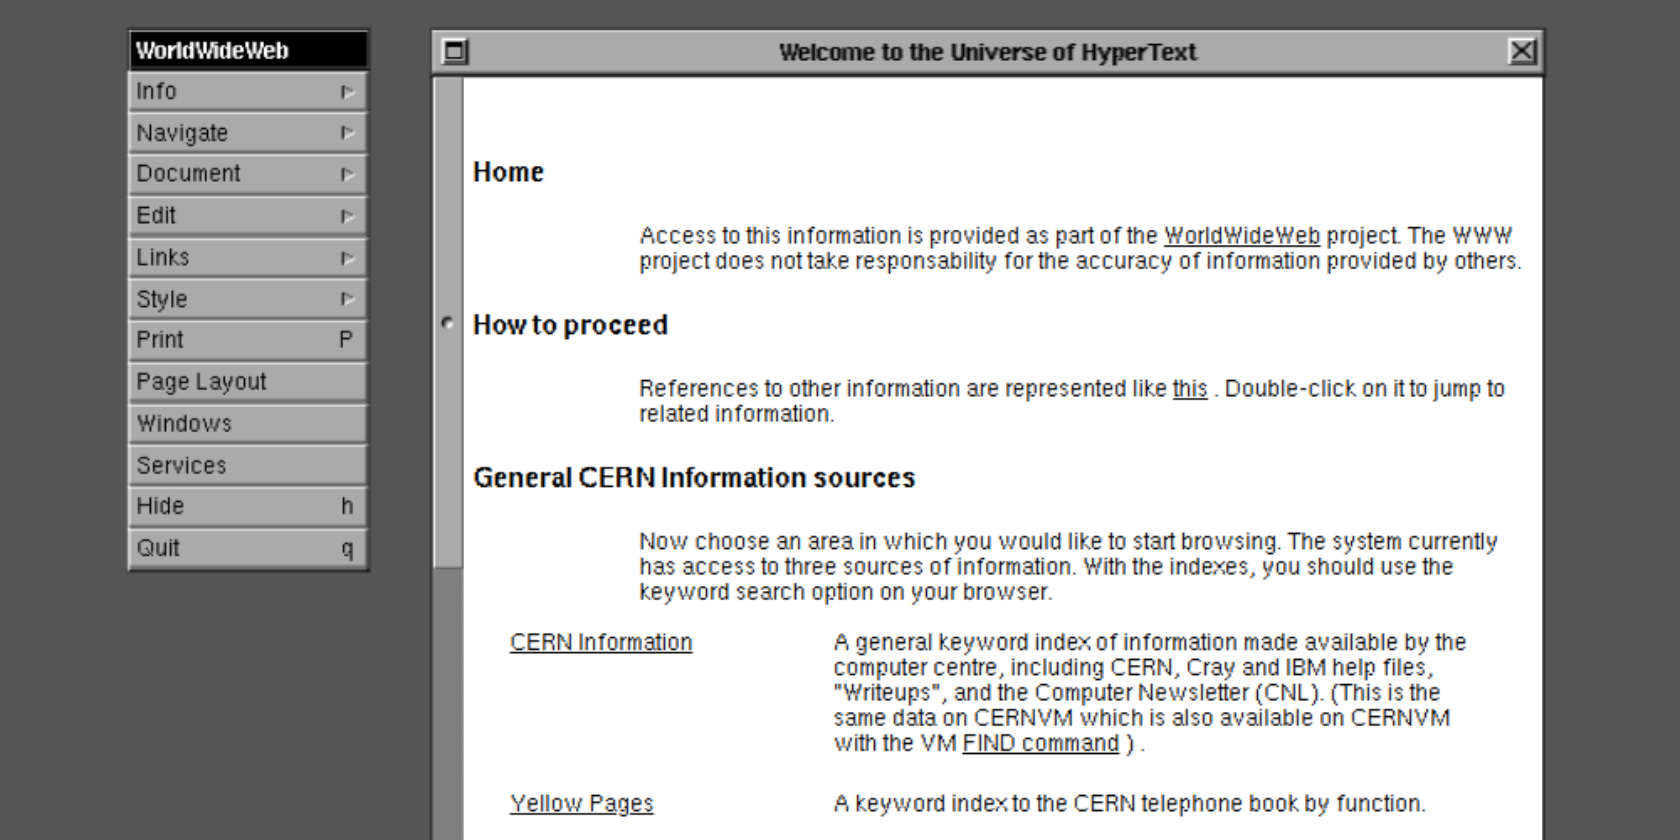
\includegraphics[width=\textwidth]{img/www-1991.png}
\end{frame}




\section{Hosting}

\begin{frameImg}[width]{img/server.jpg}
    \vspace*{60mm}
    \begin{cardTiny}
        \vspace*{\fill}
        \begin{center}
            \textbf{Hosting}
        \end{center}
    \end{cardTiny}
\end{frameImg}

\begin{frame}{Hosting}
    \begin{multicols}{3}
        \centering

        \begin{cardTiny}
            \begin{flushleft}
                \textbf{Serverhosting}

                Pronájem celého serveru.

                Zákazník má administrátorský přístup.

                Lze využívat i pro jiné účely než provozování webu.
            \end{flushleft}
        \end{cardTiny}

        \begin{cardTiny}
            \begin{flushleft}
                \textbf{Webhosting}

                Prostor pro webové stránky na cizím serveru.
            \end{flushleft}
        \end{cardTiny}

        \begin{cardTiny}
            \begin{flushleft}
                \textbf{Freehosting}

                Webhosting zdarma.

                Mohou chybět technologie, databáze a další služby.

                Často se vkládá reklama, či je jinak omezena.

                Doména 3. řádu.
            \end{flushleft}
        \end{cardTiny}
    \end{multicols}
\end{frame}

\begin{frame}{Další služby}
    \begin{cardTiny}
        \begin{flushleft}
            \textbf{Doména}.

            Databáze.

            E-maily.

            \textbf{Certifikáty}.

            Výpočetní služby.
        \end{flushleft}
    \end{cardTiny}
\end{frame}

\begin{frame}{Výběr hostingu}
    \begin{cardTiny}
        \begin{flushleft}
            Jaké funkce potřebují webové stránky k funkčnosti?

            Jak velikou návštěvnost očekáváme?

            Kolik prostoru a zdrojů zabere webová stránka?

            Jaká je důvěryhodnost poskytovatele?

            Jaká je cena hostingu?

            Jakou doménu bude webová stránka používat?
        \end{flushleft}
    \end{cardTiny}
\end{frame}

\begin{frame}{Hostingy}
    \begin{multicols}{3}
        \centering

        \begin{cardTiny}
            \begin{center}
                \textbf{Endora}
            \end{center}
        \end{cardTiny}

        \begin{cardTiny}
            \begin{center}
                \textbf{WEDOS}
            \end{center}
        \end{cardTiny}

        \begin{cardTiny}
            \begin{center}
                \textbf{Forpsi}
            \end{center}
        \end{cardTiny}

        \begin{cardTiny}
            \begin{center}
                \textbf{Active24}
            \end{center}
        \end{cardTiny}

        \begin{cardTiny}
            \begin{center}
                \textbf{Stable}
            \end{center}
        \end{cardTiny}

        \begin{cardTiny}
            \begin{center}
                \textbf{Web4U}
            \end{center}
        \end{cardTiny}
    \end{multicols}
\end{frame}

\begin{frame}{Porovnání hostingů}
    \begin{cardTiny}
        \begin{center}
            \textbf{ÚKOL}
        \end{center}
        \begin{flushleft}
            Provnejte nabídky různých \textbf{českých} hostingů. Rozhodněte, který z hostingu je dle Vás, nejvhodnější pro malé statické stránky s normální návštěvnostní, které nechtějí reklamu hostingu. Ignorujte domény. 
        \end{flushleft}
    \end{cardTiny}
\end{frame}



\section{Certifikáty}

\begin{frameImg}[width]{img/certificate.jpg}
    \vspace*{60mm}
    \begin{cardTiny}
        \vspace*{\fill}
        \begin{center}
            \textbf{Certifikáty}
        \end{center}
    \end{cardTiny}
\end{frameImg}

\begin{frame}{Certifikáty}
    \begin{cardTiny}
        \begin{flushleft}
            Určené pro jednoznačnou identifikaci entity (stránky, uživatele).
            
            Vytváří zabezpečené spojení pomocí \textbf{podepsání}.

            \vspace{2ex}

            Vydává certifikační autorita.

            Veřejný (encrypt) a soukromý (decrypt) klíč. 

            Certifikát lze získat i zdarma (Let's Encrypt). 
            
            \vspace{2ex}

            Self-signed certifikáty.

            Důvěryhodnost certifikátů.
        \end{flushleft}
    \end{cardTiny}
\end{frame}

\begin{frame}{Certifikáty}
    \begin{cardTiny}
        \begin{flushleft}
            Obsahuje důležité informace o autoritě, vydavateli, vystavení, podepsání.

            Je platný \textbf{určitou dobu} po podepsání.

            Lze zneplatnit, klient je však může přesto považovat za důvěryhodné.
            \vspace{2ex}

            Využití: HTTP\textbf{S}, VPN, SFTP, SSH, ...
        \end{flushleft}
    \end{cardTiny}

    \begin{cardTiny}
        \begin{center}
            \textbf{Jaké problémy mají certifikáty?}
        \end{center}
    \end{cardTiny}
\end{frame}

\begin{frame}
    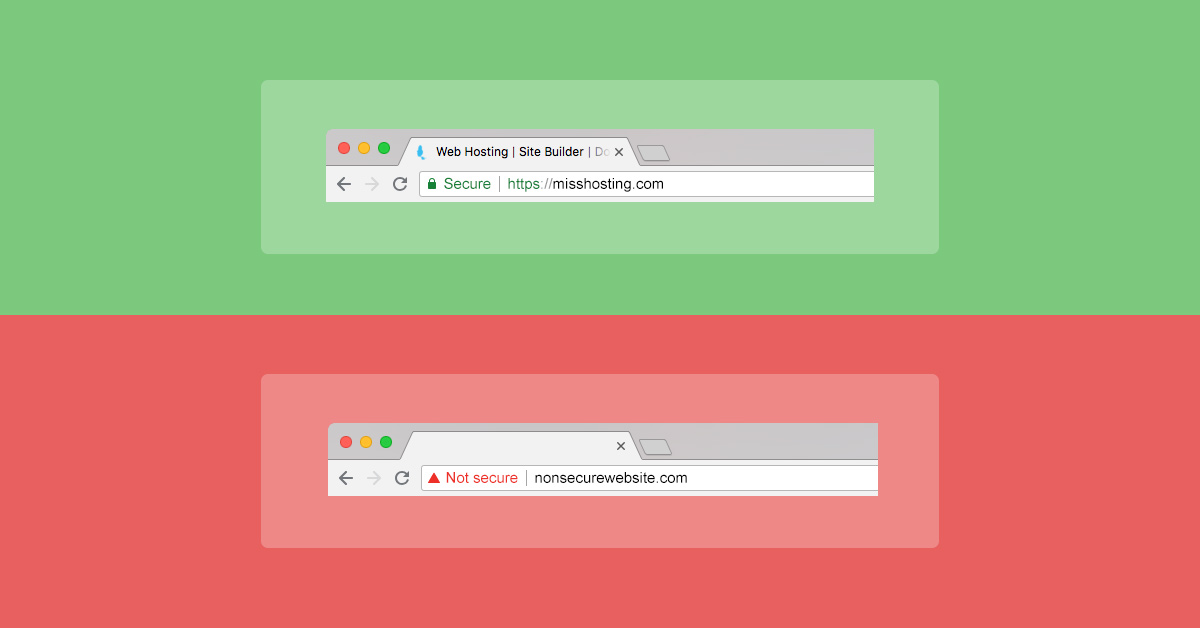
\includegraphics[width=\textwidth]{img/secure.jpg}
\end{frame}

\begin{frame}
    
\includegraphics[width=\textwidth]{img/ps.png}
\end{frame}

\begin{frameImg}{img/this-is-fine.jpg}
    \vspace*{60mm}
    \begin{cardTiny}
        \vspace*{\fill}
        \begin{center}
            \textbf{Ukázka certifikátů}
        \end{center}
    \end{cardTiny}
\end{frameImg}

\begin{frame}{Certifikáty}
    \begin{cardTiny}
        \begin{center}
            \textbf{ÚKOL}
        \end{center}
        \begin{flushleft}
            Vyberte (najděte) si jakoukoliv stránku, která využívá protokol HTTPS a prozkoumejte certifikát. Narazili jste na něco zajímavého?
        \end{flushleft}
    \end{cardTiny}
\end{frame}



\section{IDN}

\begin{frame}{IDN}
    \begin{cardTiny}
        \begin{flushleft}
            = \textbf{Internationalized Domain Names}

            Zavedení libovolných znaků do domenových jmen.

            Automaticky se převádí do ASCII podoby tzn. á $\rightarrow$ \texttt{xn--1ca}.

            Pro českou doménu je vypnuto - způsobilo by spoustu problémů.

            \href{https://xn--hkyrky-ptac70bc.cz}{http://www.háčkyčárky.cz}
        \end{flushleft}
    \end{cardTiny}
    \begin{cardTiny}
        \begin{center}
            \textbf{Proč by to způsobilo problémy?}
        \end{center}
    \end{cardTiny}
\end{frame}



\section{CMS}

\begin{frame}{CMS}
    \begin{cardTiny}
        \begin{flushleft}
            = \textbf{Content Managment System}

            Systém pro správu obsahu.

            Redakční nebo publikační systém.

            Správa webového obsahu pomocí uživatelského prostředí.

            Využívají se různé jazyky, samotné zobrazení obsahu i administrace je webová stránka.

            Např. WordPress, Joomla!, Drupal, ...
        \end{flushleft}
    \end{cardTiny}
\end{frame}



\section{Autorský zákon}

\begin{frame}{Autorský zákon}
    \begin{cardTiny}
        \begin{flushleft}
            \textbf{Webové stránky jsou chráněny autorským zákonem.}

            \vspace{2ex}
            Nemá-li něco licenci, znamená to, že to nelze bez souhlasu autora použít.

            Vždy je potřeba zkontrolovat zdroj a zda je možné danou věc použít \textbf{a za jakých podmínek}.

            \vspace{2ex}
            Creative Commons - \textbf{\href{https://www.youtube.com/watch?v=4ZvJGV6YF6Y}{video}}, \href{https://creativecommons.org/licenses/?lang=cs}{licence}
            
            \vspace{2ex}
            \textbf{Fair use}
        \end{flushleft}
    \end{cardTiny}
    \begin{cardTiny}
        \begin{center}
            \textbf{Jaké podmínky pro použití existují?}
        \end{center}
    \end{cardTiny}
\end{frame}

\begin{frame}{Zadarmo dostupné věci}
    \begin{multicols}{2}
        \centering

        \begin{cardTiny}
            \begin{flushleft}
                \textbf{Neplacené}

                \vspace{2ex}
                Fotobanky - \href{https://pixabay.com/cs/}{Pixabay}, \href{https://unsplash.com}{Unsplash}

                \vspace{2ex}
                Písma - \href{https://fonts.google.com/}{Google Fonts}
                
                \vspace{2ex}
                Ikonky - \href{https://fontawesome.com}{Font Awesome}, Flaticon
                
                \vspace{2ex}
                Freepik

                \vspace{2ex}
                Material Design, Bootstrap
            \end{flushleft}
        \end{cardTiny}
        \begin{cardTiny}
            \begin{flushleft}
                \textbf{Placené}

                \vspace{2ex}
                Fotobanky - \href{https://www.shutterstock.com/cs/}{Shutterstock}

                \vspace{2ex}
                Písma - Myfonts
                
                \vspace{2ex}
                Ikonky - Font Awesome, Steamline Icons
            \end{flushleft}
        \end{cardTiny}
    \end{multicols}
\end{frame}



\section{Shrnutí}
\begin{frame}{Shrnutí}
    \begin{cardTiny}
        \begin{center}
            \textbf{Co je to IDN a proč není povoleno na české doméně 1. řádu?}
        \end{center}
    \end{cardTiny}

    \begin{cardTiny}
        \begin{center}
        \textbf{K čemu slouží certifikáty?}
        \end{center}
    \end{cardTiny}

    \begin{cardTiny}
        \begin{center}
        \textbf{Jaký rozdíl je mezi serverhostingem a webhostingem?}
        \end{center}
    \end{cardTiny}

    \begin{cardTiny}
        \begin{center}
        \textbf{Co to je vykreslovací jádro a k čemu slouží?}
        \end{center}
    \end{cardTiny}

    \begin{cardTiny}
        \begin{center}
        \textbf{Co je to trojský kůň, Adware a Ransomware?}
        \end{center}
    \end{cardTiny}
\end{frame}


\begin{frame}{Nová verze stránky pro přípravu na test}
    \begin{cardTiny}
        \begin{center}
            \textbf{ÚKOL}
        \end{center}
        \begin{flushleft}
            Vyzkoušejte si upravené stránky \href{https://cajthaml.eu}{cajthaml.eu} a na stránce s opakováním k prvnímu testu odpovídejte na otázky.
        \end{flushleft}
    \end{cardTiny}
\end{frame}

\begin{frameImg}[width]{img/pray.jpg}
    \vspace*{60mm}
    \begin{cardTiny}
        \vspace*{\fill}
        \begin{center}
            \textbf{Písemné zkoušení}
        \end{center}
    \end{cardTiny}
\end{frameImg}

\end{document}